\chapter{作物模式}
%\addcontentsline{toc}{chapter}{作物模式}

%\begin{作物模式}
GPAM1可以模拟作物生长发育的关键过程及其对天气/气候、近地面大气$\mathrm{CO_2}$和$\mathrm{O_3}$浓度和氮沉降、
农田管理的响应和生物、化学、物理反馈。
下面详述作物区别与自然植被、需要特殊处理的过程参数化方案。

GPAM1包含64个作物功能类型(Crop Functional Type, CFT)(表~\ref{tab:CoLM预设作物功能类型}),但目前可打开使用的是14个,模拟5种作物类型: 冬小麦、春小麦、水稻、玉米、大豆(图~\ref{fig:作物功能类型覆盖率的空间分布})。每种作物类型各分雨养(rainfed)和灌溉(irrigated)CFT,玉米和大豆又分温带和热带。每个CFT占用一个水热独立的陆表单元(patch)。
{
\begin{table}[htbp]
\centering
  \caption{CoLM里预设的作物功能类型(CFT)及目前打开可模拟的CFT}
  \label{tab:CoLM预设作物功能类型}
  \begin{tabular}{@{}clc|clc@{}}
  \toprule
  Index	& CFT名称	& 打开?&	Index	& CFT名称	& 打开?\\
  \midrule
  15 &	无管理的雨养C3作物	 &   &	47	& 雨养葡萄	&  \\
  16 &	无管理的灌溉C3作物	 &  &	48 &	灌溉葡萄	&  \\
  17 &	温带雨养玉米	& \checkmark &	49	& 雨养花生 & \\	
  18 &  温带灌溉玉米	& \checkmark &	50	& 灌溉花生 & \\	
  19 &  雨养春小麦	& \checkmark & 51	& 雨养小米  & \\
  20 &  灌溉春小麦	& \checkmark & 52	& 灌溉小米  & \\
  21 & 雨养冬小麦	& \checkmark & 53	& 雨养油棕  & \\
  22 & 灌溉冬小麦	& \checkmark & 54	& 灌溉油棕  & \\
  23 & 温带雨养大豆	& \checkmark & 55	& 雨养马铃薯	& \\
  24 & 温带灌溉大豆	& \checkmark & 56	& 灌溉马铃薯	& \\
  25 & 雨养大麦 & 	& 57 &	雨养豆类	& \\
  26 & 灌溉大麦 &  & 58 &	灌溉豆类	& \\
  27 & 雨养冬大麦 &	 & 59 & 雨养油菜籽 & \\	
  28 & 灌溉冬大麦 &	 & 60 & 灌溉油菜籽 & \\	
  29 & 雨养黑麦 & 	& 61 &	雨养水稻	& \checkmark \\
  30 & 灌溉黑麦 & 	& 62 &	灌溉水稻	& \checkmark \\
  31 & 雨养冬黑麦 &	 &	63 & 雨养高粱 & \\
  32 & 灌溉冬黑麦 &	 &	64 & 灌溉高粱 & \\
  33 & 雨养木薯 &	 &	65 & 雨养甜菜 & \\
  34 & 灌溉木薯 &	 &	66 & 灌溉甜菜 & \\
  35 & 雨养柑橘 &	 &  67 & 雨养甘蔗 & \\	
  36 & 灌溉柑橘 &   &	68 & 灌溉甘蔗 & \\	
  37 & 雨养可可 &	 &	69 & 雨养向日葵 &	\\
  38 & 灌溉可可 &   &	70 & 灌溉向日葵 & \\
  39 & 雨养咖啡 &   &	71 & 雨养芒草 & \\
  40 & 灌溉咖啡 &   &	72 & 灌溉芒草 & \\
  41 & 雨养棉花 &	 &  73 & 雨养柳枝稷 & \\	
  42 & 灌溉棉花 &	 &  74 & 灌溉柳枝稷 & \\
  43 & 雨养枣椰树 &  &	75 & 热带雨养玉米	& \checkmark \\
  44 & 灌溉枣椰树 &  &	76 & 热带灌溉玉米	& \checkmark \\
  45 & 雨养牧草 &   &	77 & 热带雨养大豆	& \checkmark \\
  46 & 灌溉牧草 &   &	78 & 热带灌溉大豆	& \checkmark \\
  \bottomrule
  \end{tabular}
\end{table}
}

{
\begin{figure}[htbp]
\centering
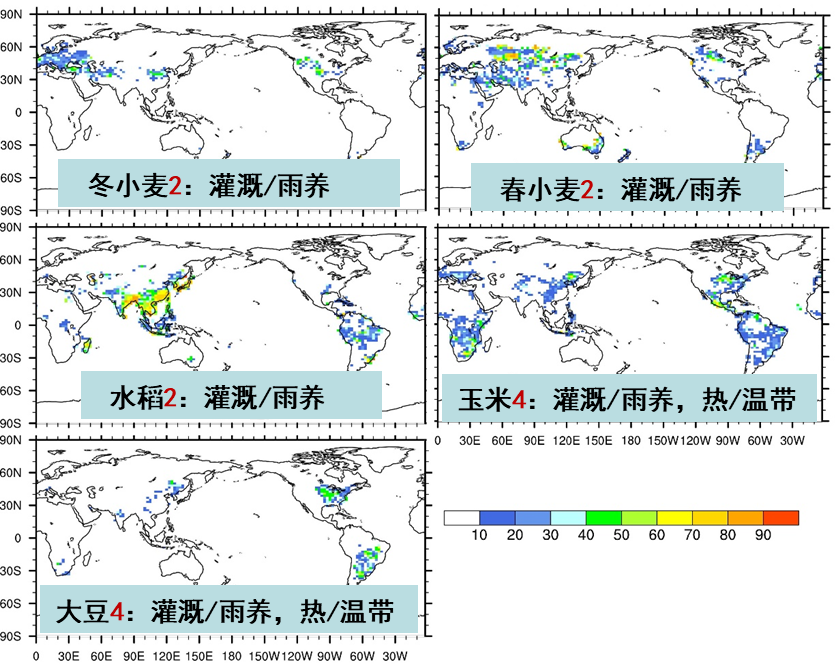
\includegraphics[scale=0.9]{Figures/作物模式/GPAM1模式模拟的14个作物功能类型格点面积覆盖率空间分布.png}
\caption{GPAM1模式模拟的14个作物功能类型(CFT)格点面积覆盖率(\%)的空间分布。}
\label{fig:作物功能类型覆盖率的空间分布}
\end{figure}
}

\section{物候}
GPAM1的物候包括三个阶段: (1)播种到抽芽; (2)抽芽到开始灌浆(grain fill); (3)灌浆到成熟/收割。所涉及的参数取值见表~\ref{tab:作物物候方案相关参数}。

% Please add the following required packages to your document preamble:
% \usepackage{booktabs}
\begin{table}[htbp]
  \centering
  \caption{作物物候方案相关参数}
  \label{tab:作物物候方案相关参数}
\begin{tabular}{@{}cccccc@{}}
\toprule
    & $T_{base}$ & $f_{LE}$  & $f_{GF}$  & $GDD_{mat}$          & $GSL_{max}$ \\ \midrule
春小麦 & 0     & 0.07 & 0.60 & 0.2$GDD_{10yr}$+1458 & 150    \\
冬小麦 & 0     & 0.03 & 0.67 & 0.38$GDD_{10yr}$+526 & 270    \\
水稻1 & 10    & 0.12 & 0.68 & 0.30$GDD_{10yr}$+695 & 150    \\
水稻2 & 10    & 0.35 & 0.75 & 0.27$GDD_{10yr}$+575 & 150    \\
玉米  & 8     & 0.11 & 0.64 & 0.26$GDD_{10yr}$r+907 & 150    \\
大豆  & 10    & 0.15 & 0.69 & 0.26$GDD_{10yr}$+802 & 150    \\ \bottomrule
\end{tabular}
\end{table}

\subsection{播种}\label{sec:播种}
  播种日期是给定的,采用全球播种日再分析数据~\citep{jagermeyr2021climate}),并结合陆表数据中的作物分布制作而成 (图~\ref{fig:GPAM1播种日空间分布}),为GPAM1的输入场。

{
\begin{figure}[htbp]
\centering
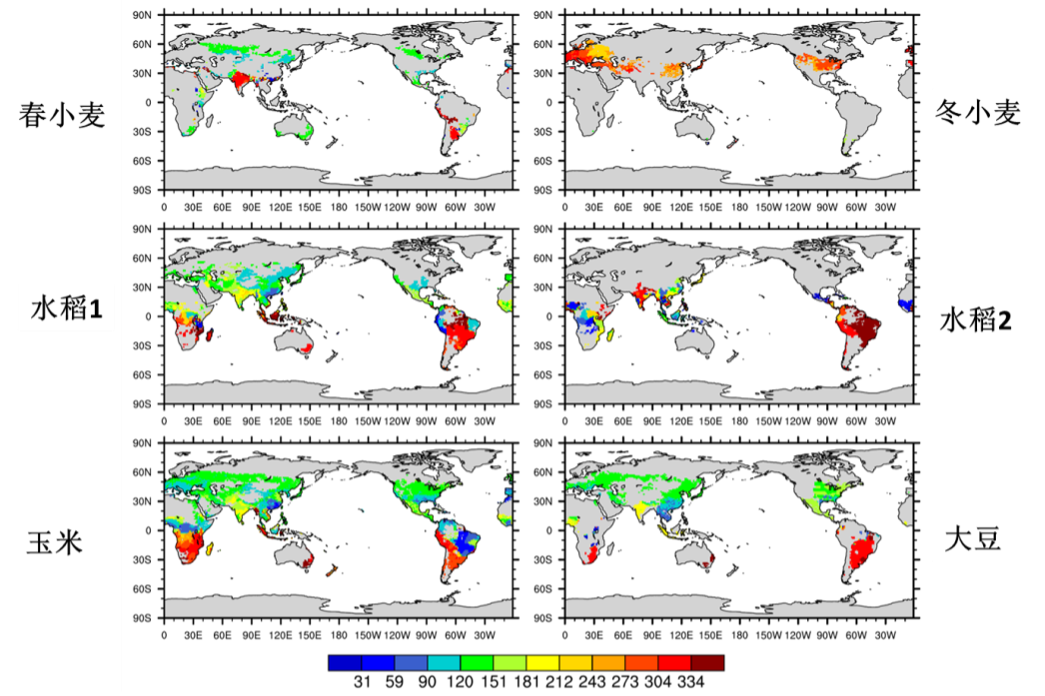
\includegraphics[scale=1.2]{Figures/作物模式/GPAM1播种日空间分布.png}
\caption{GPAM1播种日空间分布。}
\label{fig:GPAM1播种日空间分布}
\end{figure}
}

\subsection{抽芽}
  当热单元指数(Heat Unit Index, $HUI$):
  \begin{equation}\label{HUI}
  HUI=\frac{GDD_{base}}{GDD_{mat}}
  \end{equation}
  达到$f_{LE}$时,开始抽芽。$GDD_{base}$是基于陆表气温的积温(\textcelsius\ days):
  \begin{equation}
  GDD_{ {base }}=\sum_{planting}^{current\ day} \min \left(0, T_{sa}-T_{base}\right)
  \end{equation}
 其中,$T_{sa}$是日地表气温,$T_{base}$是底温(作物在该温度下停止生长)。
  
\subsection{灌浆}
  当$HUI$达到$f_{GF}$时,开始灌浆。

\subsection{成熟}
  当$HUI$达到1时或生长季达到最长生长季长度$GSL_{max}$时,作物成熟。其中,$GDD_{mat}$是$GDD_{base}$ 
  10年滑动平均的一元线性方程(表~\ref{tab:作物物候方案相关参数})。
  \begin{equation}
    GDD_{mat}=a GDD_{10yr}+b
  \end{equation}
  
\subsection{收割}
  假设达到成熟的时步收割。


\section{生理变化}
作物的碳(C)库和氮(N)库有leaf, live stem, grain, fine root库及相应的transfer和storage库,无dead stem, live coarse root, dead coarse root库及相应的transfer和storage库。由于新加了grain库,相应通量会增加分配到grain的C/N通量,grain到Aproduct及litter的C/N通量。作物的呼吸和周转与草相同。

\subsection{光合和气孔导度}
大豆、小麦、水稻采用C3植物光合方案;玉米采用C4植物光合方案。
在基于Medlyn方案计算气孔导度时,玉米的参数取值$g_1=1.8$,低于自然植被,其余作物的参数取值$g_1=5.8$,高于自然植被。该参数越大,气孔导度越高。

\subsection{分配}
分配系数随物候阶段变化而变化。从出叶开始,按下列分配系数公式分配到叶库Cleaf,茎库Cleaf,根库Croot,粒库Cgrain。
不同物候期分配系数见表~\ref{tab:作物分配方案相关参数}。

(1)	物候期2 \\
\begin{equation}
\left\{\begin{array}{c}
  a_{grain}=0 \\ 
  a_{root}=a_{root\_i}-\left(a_{root\_i}-a_{root\_f}\right) HUI \\
  a_{leaf}=\left(1-a_{root}\right) a_{leaf\_i} \frac{{e}^{-{b}}-{e}^{-b \frac{HUI}{f_{GF}}}}{{e}^{-{b}}-1}   \\
  a_{stem}=1-a_{grain}-a_{root}-a_{leaf}
  \end{array}\right.
\end{equation}
其中,下标$i$和$f$表示该分配系数的初值和终值,$b=0.1$。

(2)	物候期3 \\
\begin{equation}
  \left\{\begin{array}{c}
    a_{leaf}=0.0 \\ 
    a_{root}=a_{root\_i}-\left(a_{root\_i}-a_{root\_f}\right) \min(1, HUI) \\
    a_{stem}=\max \left[a_{stem\_f}, a_{stem} \max \left(0, \frac{1-HUI}{1-f_{GF}}\right)^{d_{sem}}\right] \\
    a_{grain}=1-a_{root}-a_{leaf}-a_{stem}
  \end{array}\right.
\end{equation}
% Please add the following required packages to your document preamble:
% \usepackage{booktabs}
\begin{table}[htbp]
  \centering
  \caption{作物分配方案相关参数}
  \label{tab:作物分配方案相关参数}
\begin{tabular}{@{}lcccc@{}}
  \toprule
参数       & 小麦   & 水稻   & 玉米   & 大豆   \\ \midrule
$\alpha_{leaf\_i}$ & 0.9  & 0.75 & 0.8  & 0.85 \\
$\alpha_{root\_i}$ & 0.1  & 0.1  & 0.4  & 0.2  \\
$\alpha_{root\_f}$ & 0    & 0    & 0.05 & 0.2  \\
$\alpha_{stem\_f}$ & 0.05 & 0.05 & 0.0  & 0.3  \\
$d_{stem}$    & 1    & 1    & 2    & 5   \\\bottomrule
\end{tabular}
\end{table}

\subsection{氮循环}
作物的氮循环和自然植被类似,但碳氮比(CN)不同。CoLM采用的作物不同组织的碳氮比CN如表~\ref{tab:作物碳氮比}所示。其中,碳氮比CNleaf, CNstem, CNroot用于灌浆前,其余碳氮比用于灌浆开始后。

此外,我们考虑了大豆根瘤中的根瘤菌与大豆共生固氮,大豆共生固氮能力设为自然植物的4倍,假设其余作物类型无生物共生固氮能力。生物共生固定的氮直接直接到 $\mathrm{NO_3^-}$ 库。

%(1) 碳氮比(CN)\\
%表~\ref{tab:作物碳氮比} 中,碳氮比$CN_{leaf}$,$ CN_{stem}$, %$CN_{root}$用于灌浆前,其余碳氮比用于灌浆开始后。\\
% Please add the following required packages to your document preamble:
% \usepackage{booktabs}
\begin{table}[htbp]
  \centering
  \caption{作物碳氮比}
  \label{tab:作物碳氮比}
\begin{tabular}{@{}lcccc@{}}
\toprule
参数         & 小麦  & 水稻  & 玉米  & 大豆  \\ \midrule
$CN_{leaf}$     & 20  & 20  & 25  & 20  \\
$CN_{stem}$     & 50  & 50  & 50  & 50  \\
$CN_{root}$     & 42  & 42  & 42  & 42  \\
$CN_{leaf\_f}$  & 65  & 65  & 65  & 65  \\
$CN_{stem\_f}$  & 100 & 100 & 120 & 130 \\
$CN_{root\_f}$  & 40  & 40  & 0   & 0   \\
$CN_{grain\_f}$ & 50  & 50  & 50  & 50  \\ \bottomrule
\end{tabular}
\end{table}

%(2) 大豆共生固氮 (SNF)\\
%考虑大豆根瘤中的根瘤菌与大豆共生固氮,大豆共生固氮能力设为自然植物的4倍,假设其余作物类型无生物共生固氮能力。生物共生固定的氮直接被植物吸收。\\
%

%\section{光合作用和气孔导度}
%大豆、小麦、水稻采用C3植物光合方案;玉米采用C4植物光合方案。
%在基于Medlyn方案计算气孔导度时,玉米的参数取值$g_1=1.8$,低于自然植被,其余作物的参数取值$g_1=5.8$,高于自然植被。该参数越大,气孔导度越高。
%


\subsection{冬小麦春化现象}
春化响应$V$(0$\sim$1)采用~\citet{streck2003incorporating}方案:
\begin{equation}
V=\frac{D_{v}{ }^{5}}{22.5^{5}+D_{v}^{5}}
\end{equation}
其中,$D_v$是物候阶段2累积的日春化率:
\begin{equation}\label{D_v_a}
D_{v}=\sum R_{v}
\end{equation}
在公式(\ref{D_v_a})中,$R_{v}$是日地表温度的函数:
\begin{equation}
R_{v} = \begin{cases} 
\frac{\left[2\left(T-T_{min}\right)^{a}\left(T_{opt}-T_{min}\right)^{a} - \left(T-T_{min}\right)^{2a}\right]}{\left(T_{opt}-T_{min}\right)^{2a}}, &T_{min} \leq T \leq T_{max} \\
0,  &T<T_{min} \quad  \text{or} \quad T>T_{max}
\end{cases}
\end{equation}
其中,$T_{min}$= –1.3 \textcelsius, $T_{opt}$= 4.9 \textcelsius, $T_{max}$= 15.7 \textcelsius。$ R_v$ 的取值从 0 (当$ T\leq T_{min}$ 或者 $ \geq  T_{max}$) 到 1 ( 当$T=T_{opt}$)。
\begin{equation}
a=\frac{\ln 2}{\ln \left[\left(T_{\max }-T_{\min }\right) /\left(T_{o p t}-T_{\min }\right)\right]}
\end{equation}

春化响应用于调整$GDD_{base}$和粒分配系数
\begin{equation}
G D D_{b a s e}=G D D_{b a s e,  { unadjusted }} \times V
\end{equation}
\begin{equation}
a_{ {grain }}=a_{ {grain,unadjusted }} \times V_{f}
\end{equation}


\section{胁迫}
\subsection{臭氧污染胁迫}
%\section{臭氧污染胁迫}
考虑臭氧对光合速率和气孔导度的影响因子 $F_{O3\_A}$ 以及$F_{O3\_{gs}}$:
\begin{equation}
F_{O3\_{A}}=-0.0022 POD_{0.5}+0.868
\end{equation}
\begin{equation}
F_{O3\_{gs}}=-0.00096 POD_{0.5}+0.856
\end{equation}
其中,$POD_{0.5}$ (Phytotoxic ozone does above a threshold of 0.5 \unit{nmol.m^{-2}.s^{-1}}, 单位:\unit{mmol.m^{-2}})是植物吸收的$O_3$通量在抽芽后生长季白天的累积量。第 $t$ 时间步的 $\mathrm{O_3}$ 通量累积量:
\begin{equation}\label{eq:POD05}
POD_{0.5,t}=POD_{0.5,t-1}\left(1-D_t\right)+U_{0.5,t} \times 10^{-6}.
\end{equation}
在公式\eqref{eq:POD05}中,$D_t$是$t$时步的$\mathrm{O_3}$通量累积量衰减率:
\begin{equation}
D_t = \max\left(0, 1-\frac{LAI_{t-1}}{LAI_t} \right),
\end{equation}
$t$ 时步的$\mathrm{O_3}$通量累积量:
\begin{equation}
U_{Y,t}=\begin{cases}
    \Delta t\times\max(F_{O3,t}-Y, 0) & \text{白天} \\
    0 & \text{其它时间}
\end{cases},
\end{equation}
其中 $\Delta t$ 是时间步长 (s); 而 $t$ 时步的$\mathrm{O_3}$通量:
\begin{equation}
    F_{O3,t}=\frac{\mathrm{[O_3]}}{r_b + r_{am} + r_sk_{O3}},
\end{equation}
其中$\mathrm{[O_3]}$ 为陆面参考高度大气的臭氧浓度(\unit{nmol.m^{-3}}), $r_{am}$ (\unit{s.m^{-1}})、$r_b$ (\unit{s.m^{-1}}) 和 $r_s$ (\unit{s.m^{-1}}) 分别为空气动力学阻抗、大气边界层阻抗、叶气孔阻抗,$k_{O3}=0.663$ 为臭氧和水蒸气的扩散比。

上面计算的$F_{{O3}\_A}$ 以及$F_{O3_{gs}}$分别作用在Farquhar--Collatz方案计算的光合速率以及Ball--Berry方案计算出的气孔导度。

\subsection{热胁迫}
作物对热胁迫的敏感期大约是在开花前后及灌浆期,在GPAM1里设为$HUI $满足$0.5 \leq HUI \leq 0.8$的时段。在每个发生热胁迫的时步,采用场数损失率$l$:
\begin{equation}
l=\left\{\begin{array}{cc}1-\left(\frac{4.3}{10.4}\right)^{\frac{\Delta t}{3600\times 21}} & T>T_{c} \\ 0 & T \leq T_{c}\end{array}\right.
\end{equation}
其中,$\Delta t$ 是时步长,$T$是该时步的温度;$T_c$是临界温度:$T_c=34$ \textcelsius (水稻,玉米,冬小麦),31 \textcelsius (春小麦),37 \textcelsius (大豆)。
每个时步考虑了热胁迫后的叶$C_{leaf}$库为:
\begin{equation}
C_{leaf}=C_{leaf,  {unadjusted}} \times (1-l)
\end{equation}


\section{管理}
\subsection{施肥}
氮肥考虑了工业氮肥和粪肥。工业氮肥是输入场。粪肥设为2 \unit{g.N.m^{−2}.yr^{−1}}。施肥时直接将氮肥输入土壤 $\mathrm{NH_4^+}$ 库,从出叶开始,以匀速的方式施肥 20 天。

\subsection{收割和农业残留物处理}
收割时粒库 $\mathrm{C_{grain}}$ 进入种子库 $\mathrm{C_{seed}}$ 和食品库 $\mathrm{C_{food}}$
\begin{equation}
\mathrm{{C}_{seed}}=\min \left(\mathrm{C_{grain}}, 3\right)
\end{equation}
\begin{equation}
\mathrm{C_{food}}=\mathrm{C_{grain}}-\mathrm{C_{seed}}
\end{equation}
其中,种子库$\mathrm{C_{seed}}$在下一个生长季出叶期的第一时步转移到叶库$\mathrm{C_{leaf}}$。叶和茎的碳库进入地上凋落物库。根的碳库进入地下凋落物库。

\subsection{秸秆焚烧及排放}
秸秆焚烧燃烧面积百分率$BAF$(\unit{s^{-1}}):
\begin{equation}
    BAF= a_1 f_{se} f_{crop}
\end{equation}
其中,$a_1$ (\unit{s^{-1}})是全球常数;$f_{se}$ 是社会经济因子的影响:
\begin{equation}
    f_{se} = f_d f_e
\end{equation}
其中,
\begin{equation}
    f_d = 0.04 + 0.96\exp\left[-\pi\left(\frac{D_p}{350}\right)\right]
\end{equation}
\begin{equation}
    f_e = 0.01 + 0.99\exp\left[-\pi\frac{GDP}{10}\right]
\end{equation}
$D_p$ (\unit{person.km^{-2}}) 及 $GDP$ (\unit{k\ 1995\ US\$.capita^{-1}})
分别是人口密度和生产总值。
$f_{crop}$ 用于判断火发生时间(发生时为1,其余时步为0),
是输入场,定义为观测播前观测的秸秆焚烧峰值时步。
观测的秸秆焚烧峰值时步基于GFED4s的3小时数据;播种时间见章节~\ref{sec:播种}。

在得到燃烧面积后,火灾引起的碳排放$CE$ (\unit{g.C.m^{-2}.s^{-1}}) 为:
\begin{equation}
CE=BAF \times C_{ab,litter} \times CC
\end{equation}
$C_{ab,litter}$是地上凋落物碳库, $CC=0.8$是燃烧完全因子。

此后,我们估算火灾引起的33种痕量气体和气溶胶排放。火灾引起的第$i$类痕量气体和气溶胶排放量$E_i$ (\unit{g.species.m^{-2}.s^{-1}}):
\begin{equation}
E_{i}=EF_{i} \times CE /[{C}]
\end{equation}
$EF_i$ (\unit{g.species.(kg.dry\ matter(DM))^{-1}})是排放因子,见表~\ref{tab:秸秆焚烧排放因子取值}。$[C]=$ \qty{0.5e3}{g.C.(kg.DM)^{-1}}是单位转换因子。


% Please add the following required packages to your document preamble:
% \usepackage{booktabs}
\begin{table}[htbp]
  \centering
  \caption{秸秆焚烧排放因子取值(\unit{g.species.(kg.DM)^{-1}})}
  \label{tab:秸秆焚烧排放因子取值}
  \begin{tabular}{@{}lc|lc@{}}
  \toprule
  种类 & 排放因子 & 种类                     & 排放因子 \\ \midrule
  CO2                    & 1421 & C2H4   (ethylene)      & 1.14 \\
  CO                     & 78   & C3H6   (propylene)     & 0.48 \\
  CH4                    & 5.9  & C5H8   (isoprene)      & 0.18 \\
  NMHC                   & 5.8  & C10H16   (terpenes)    & 0.03 \\
  H2                     & 2.65 & C7H8   (toluene)       & 0.18 \\
  NOx                    & 2.67 & C6H6   (benzene)       & 0.31 \\
  N2O                    & 0.09 & C8H10   (xylene)       & 0.09 \\
  PM2.5                  & 8.5  & CH2O   (formaldehyde)  & 1.80 \\
  TPM                    & 11.3 & C2H4O   (acetaldehyde) & 1.82 \\
  TPC                    & 5.5  & C3H6O   (acetone)      & 0.61 \\
  OC                     & 5.0  & C3H6O2(hydroxyacetone) & 1.74 \\
  BC                     & 0.43 & C6H5OH   (Phenol)      & 0.50 \\
  SO2                    & 0.81 & NH3 (ammonia)          & 1.04 \\
  C2H6   (ethane)        & 0.76 & HCN (hydrogen cyanide) & 0.43 \\
  CH3OH   (methanol)     & 2.63 & MEK/2-butanone         & 0.60 \\
  C3H8   (propane)       & 0.20 & CH3CN   (acetonitrile) & 0.25 \\
  C2H2   (acetylene)     & 0.32 &                        &      \\ \bottomrule
  \end{tabular}
\end{table}


\subsection{灌溉}
CoLM灌溉方案基于\citet{ozdogan2010simulating} 和 \citet{yao2022Irrigation}方案,在灌溉作物种类的播种区考虑。

CoLM灌溉模块主要分为三部分:计算潜在灌溉需求水量;计算灌溉供应水量;计算灌溉施加水通量,实现对灌溉过程的模拟。考虑到实际灌溉方式在全球存在显著差异,因此每种作物在不同网格分别采用了滴灌、喷灌、漫灌、稻田灌溉四种不同的灌溉方式。

当地时间每天早上6点,模块将判断是否有正在生长的灌溉作物,如果存在,则将逐步计算灌溉需求量、灌溉供应量以及灌溉施加。

首先,计算潜在灌溉需求水量(mm):
\begin{equation}
    D_{irrig} = \begin{cases}
        \omega_{irrig} - \omega_{avail} & \omega_{thresh} > \omega_{avail} \\
        0     & \omega_{thresh} \leq \omega_{avail}
    \end{cases},
\end{equation}
其中,$\omega_{avail}$ 为土壤当前总水量(mm):
\begin{equation}\label{eq:omega-avail}
    \omega_{avail} = \sum_{j=1}^{N_{irr}}\theta_j\Delta z_j;
\end{equation}
$\omega_{irrig}$ 为实际灌溉目标水量(mm):
\begin{equation}
    \omega_{irrig} = f_{thresh}(\omega_{target}-\omega_{wilt}) + \omega_{wilt}, 
\end{equation}
其中,$\omega_{target}$ 为灌溉目标水量(mm): 
\begin{equation}
    \omega_{target} = \sum_{j=1}^{N_{irr}}\theta_{target}\Delta z_j,
\end{equation}
$\omega_{wilt}$ 为萎蔫点土壤水量(mm):
\begin{equation}\label{eq:omega-wilt}
    \omega_{wilt} = \sum_{j=1}^{N_{irr}}\theta_{wilt}\Delta z_j.
\end{equation}
方程\eqref{eq:omega-avail}--\eqref{eq:omega-wilt}中,$N_{irr}$ 为发生灌溉土壤层数,与设定灌溉深度$z_{irrig}$有关;$\Delta z_j$ 为第$j$层土壤厚度;$\theta_{target}$、$\theta_{wilt}$和$\theta_j$ 则分别为土壤各层的灌溉目标湿度、田间萎蔫点以及土壤实际湿度,需要根据其对应的土壤水势$\Phi_{target}$、 $\Phi_{wilt}$和$\Phi_j$ 计算。

由于不同灌溉方式的触发灌溉阈值和目标灌溉量存在差异,灌溉触发阈值为:
\begin{equation}
    \omega_{thresh} = f_{thresh}(\omega_{trigger}-\omega_{wilt}) + \omega_{wilt},
\end{equation}
其中 $\omega_{trigger}$ 为触发灌溉的目标水量,根据 $\Phi_{trigger}$ 计算,$f_{thresh}$ 为灌溉调优参数,$\omega_{thresh}$ 为触发灌溉水量阈值。相应的灌溉方案参数见表~\ref{tab:灌溉方案参数}。

\begin{table}[htbp]
  \centering
  \caption{灌溉方案参数}
  \label{tab:灌溉方案参数}
  \begin{threeparttable}
  \begin{tabular}{@{}ccccc}
  \toprule
        & drip   & sprankler   & flood   & paddy   \\ \midrule
$f_{thresh}$ & 1  & 1 & 1  & 1 \\
$z_{irrig}(m)$ & 0.6  & 0.6  & 0.6  & 0.6  \\
$\Phi_{target}$(mm) & -3300    & -3300  & $\Phi_0$ & $\Phi_0$  \\
$\Phi_{trigger}$(mm) & -3300 & -3300 & -3300  & $\Phi_0$  \\
$\Phi_{wilt}$ (mm)   & -150000    & -150000    & -150000    & -150000   \\\bottomrule
\end{tabular}
\begin{tablenotes}
    \footnotesize
    \item[注:] $\Phi_0$ 为饱和水势。
\end{tablenotes}
\end{threeparttable}    
\end{table}

计算灌溉供应水量,假设灌溉需求灌溉量可全部被地下水提供。

计算灌溉施加水通量时,考虑到实际灌溉策略,假定灌溉发生后,实际灌溉水量将在4小时内,根据灌溉方式均匀施加。其中喷灌施加在作物冠层,经历冠层截留到达地表;而其他灌溉方式则直接将水施加在地表。

灌溉速率$R_{irrig}$ 为:
\begin{equation}
    R_{irrig} = \frac{D_{irrig}}{T_{irrig}},
\end{equation}
其中,$T_{irrig}$ 为灌溉持续时间(默认值14400 s)。
\section{结构形态}
出叶后到收割前,叶面积为:
\begin{equation}
LAI=C_{leaf} \times SLA
\end{equation}
SLA为比叶面积 (\unit{m^2.leaf.g^{-1}.C})(表~\ref{tab:结构形态参数})。

茎叶面积为:
\begin{equation}
SAI=\left\{\begin{array}{lcc}0.1 LAI, & \text { for } & \text { maize } \\
   0.2 LAI, & \text { for } & \text {others}\end{array}\right.
\end{equation}

冠层顶高度$z_{top}$(米)和冠层底高度$z_{bot}$(米)为:
\begin{equation}
z_{top}=\max \left[0.05, z_{top,max} \min \left(\frac{HUI}{f_{GF}}, 1.0\right)\right]
\end{equation}
\begin{equation}
z_{b o t}=0.02
\end{equation}

% Please add the following required packages to your document preamble:
% \usepackage{booktabs}
\begin{table}[htbp]
  \centering
  \caption{结构形态参数}
  \label{tab:结构形态参数}
  \begin{tabular}{@{}lccccc}
  \toprule
  参数   & 春小麦  & 冬小麦 & 水稻    & 玉米   & 大豆    \\ \midrule
  $SLA$  & 0.0453 & 0.0441 & 0.0431 & 0.0409 & 0.0566 \\
  $z_{top,max}$ & 0.808 & 0.852 & 0.98 & 2.55 & 0.823     \\ \bottomrule
  \end{tabular}
\end{table}
